\chapter{Desarrollo de la interfaz web}\label{chapter:Desarrollo de la interfaz web}

		Luego de garantizar el flujo correcto de la información de un componente a otro, surgió la necesidad de desarrollar una extensión del sistema, con una interfaz web que facilitara su uso para los clientes finales. Del mismo modo, dicha interfaz permite el ingreso de usuarios que compran el servicio de Internet del hotel.
\newline
\newline
\indent En el presente capítulo se presentan: en la primera sección la arquitectura usada para el desarrollo de la aplicación; en la segunda sección se listan los casos de usos que describen las actividades posibles a realizar en la aplicación; en la tercera sección se definen los \textit{stakeholders} del sistema. En la cuarta sección presenta el Diagrama de casos de Uso de la apliación. En la quinta sección se detallan los requerimientos no funcionales del sistema; y, finalmente, en la sexta sección se resumen los resultados obtenidos en esta fase del proyecto.

\section{Arquitectura de la aplicación} \label{sect:Arquitectura de la aplicacion}
		El prototipo fue desarrollado como aplicación web, utilizando el patrón arquitectónico Modelo-Vista-Controlador (MVC), provisto por el framework de desarrollo escogido: Django.
\newline
\newline		
\indent De esta manera, en el modelo se representan las tablas provistas por FreeRadius, y las añadidas en el desarrollo de NetPass. El controlador responde a las acciones del usuario e invoca peticiones al modelo al realizarse una solicitud sobre usuarios de la red (por ejemplo, listar usuarios actuales). La vista presenta el modelo a través de una interfaz amigable e intuitiva, permitiendo al usuario final disparar acciones.
		
		En la figura ~\ref{fig:mvc} se muestra el diagrama que representa la estructura del patrón MVC. Los componentes interactúan a través de invocaciones (línea continua) y eventos (línea de trazos).


\begin{figure}[ht]
  \centering
  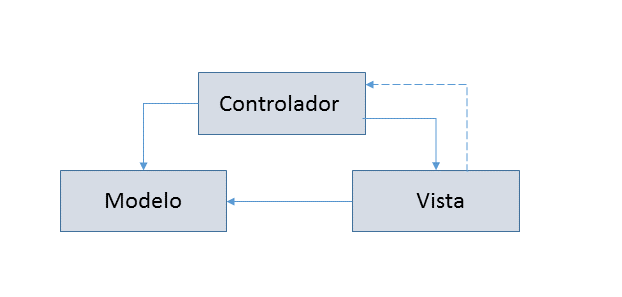
\includegraphics[scale=0.6,type=png,ext=.png,read=.png]{imagenes/mvc} \\
  \centering
  \caption{Diagrama del patrón arquitectónico MVC.}
  \label{fig:mvc}
\end{figure}


\section{Casos de uso} \label{sect:Casos de usos}
		Una especificación completa de estas historias puede ser revisada en el apéndice B.


\section{\textit{Stakeholders}} \label{sect:Stakeholders}
		Se puede definir \textit{stakeholder} como cualquier persona o entidad que es afectada o concernida por las actividades o la marcha de una organización \cite{MTSH}. En este caso, los afectados con el desarrollo de este proyecto son: 
\newline
\indent Los usuarios del sistema, que se clasifican en dos: Gerente de sistemas del hotel, y personal de front-desk (recepción del hotel). El primero tiene priviliegios de superusuario en el sistema, lo que le permite realizar acciones extras. 
\newline
\indent Los usuarios de la red, es decir, lo huéspedes del hotel o aquellos usuarios que compran el servicio de Internet. 

\section{Diagrama de Casos de Uso} \label{sect:Casos de uso}
En la Figura ~\ref{fig:UseCases} se presenta el diagrama de casos de uso de NetPass. 

\begin{figure}[ht]
  \centering
  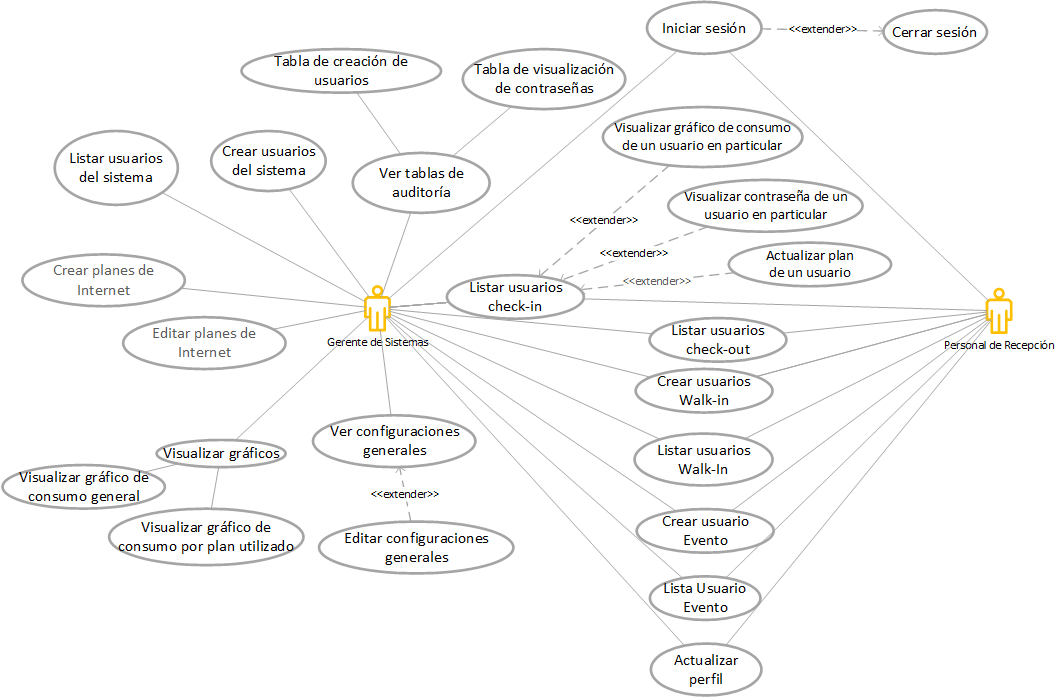
\includegraphics[scale=0.6,type=png,ext=.png,read=.png]{imagenes/UseCases} \\
  \caption{Diagrama de casos de uso de NetPass.}
  \label{fig:UseCases}
\end{figure}

\section{Requerimientos no funcionales} \label{sect:Requerimientos no funcionales}
\subsection{Seguridad}
		El sistema cuenta con una serie de características que lo convierten en una pieza de software seguro. Se hizo especial énfasis en la seguridad de urls, es decir, que el ingreso de algún url forzado en el navegador redireccionara según los privilegios de cada usuario. De igual forma, los archivos (tanto del frontend como del backend del sistema) pertenecen a un usuario creado en la máquina en la que se aloja el sistema, con permisos de lectura y escritura exclusivos para el propietario.

\subsection{Eficiencia}
		El sistema es capaz de procesar múltiples ‘mensajes’ en un tiempo de respuesta de menos de 5 segundos, y en el orden en el que estos sean enviados por la interfaz. El diseño del software está hecho de tal manera que la conexión con ambos entes (interfaz y el software de autenticación) sea permanente, a la espera de cualquier mensaje para procesar, a cualquier hora del día, y que dicha conexión no sea vulnerable a cualquier excepción que pueda surgir.

\subsection{Usabilidad}
		La interfaz web implementada es simple, amigable e intuitiva, lo que incrementa la facilidad de aprendizaje para los usuarios finales del sistema. Se hace especial énfasis en la simpleza de la interfaz, ya que de esta manera se maximiza la velocidad de las operaciones. Se implementaron también, métodos de minimización de la taza de errores, por ejemplo, mensajes de confirmación para cada acción (en especial, las que involucran manejo de dinero). 

\subsection{Portabilidad}
		El sistema fue diseñado para alojarse en una distribución Linux, con ciertos requerimientos mínimos para su correcta ejecución (descritos en capítulos siguientes). La aplicación web por su parte, es ejecutable en distintos navegadores, tales como Chrome, Firefox, Microsoft Edge, entre otros.

\section{Resultados obtenidos} \label{sect:Resultados obtenidos}
		Como resultado de esta etapa del desarrollo se obtuvo la extensión del sistema NetPass, es decir, la interfaz web que acompaña al backend de la aplicación. Dicha interfaz permite registrar nuevos usuarios en función de que tengan acceso a la red, visualizar los que están ya registrados, y modificar ciertos parámetros configurables. Es también, amigable e intuitiva lo que permite al usuario utilizarla, incrementando su grado de familiarización.
		
\section{Pruebas}
		Las pruebas correspondientes a esta etapa del desarrollo consistieron en la ejecución de cada caso de uso de la aplicación. En caso de no obtener los resultados esperados, se aplicaban los cambios pertinentes. Dicho trabajo fue realizado por miembros de la empresa involucrados en el proyecto.